\section{Performance Measurements and Results}

\subsection{Performance metrics}
There are four common performance metrics 
\begin{itemize}
    \item Execution time:
    \item Memory-consumption \& number of machines:
    \item Solution quality:
\end{itemize}

\subsection{Result of recent four decades}

Same as Milestone $3$, we selected the year 1983, 1993, 2003 and 2013 to show the results.

150 clusters, 500 iterations.

\begin{figure}
    \centering
    \begin{tabular}{c}
        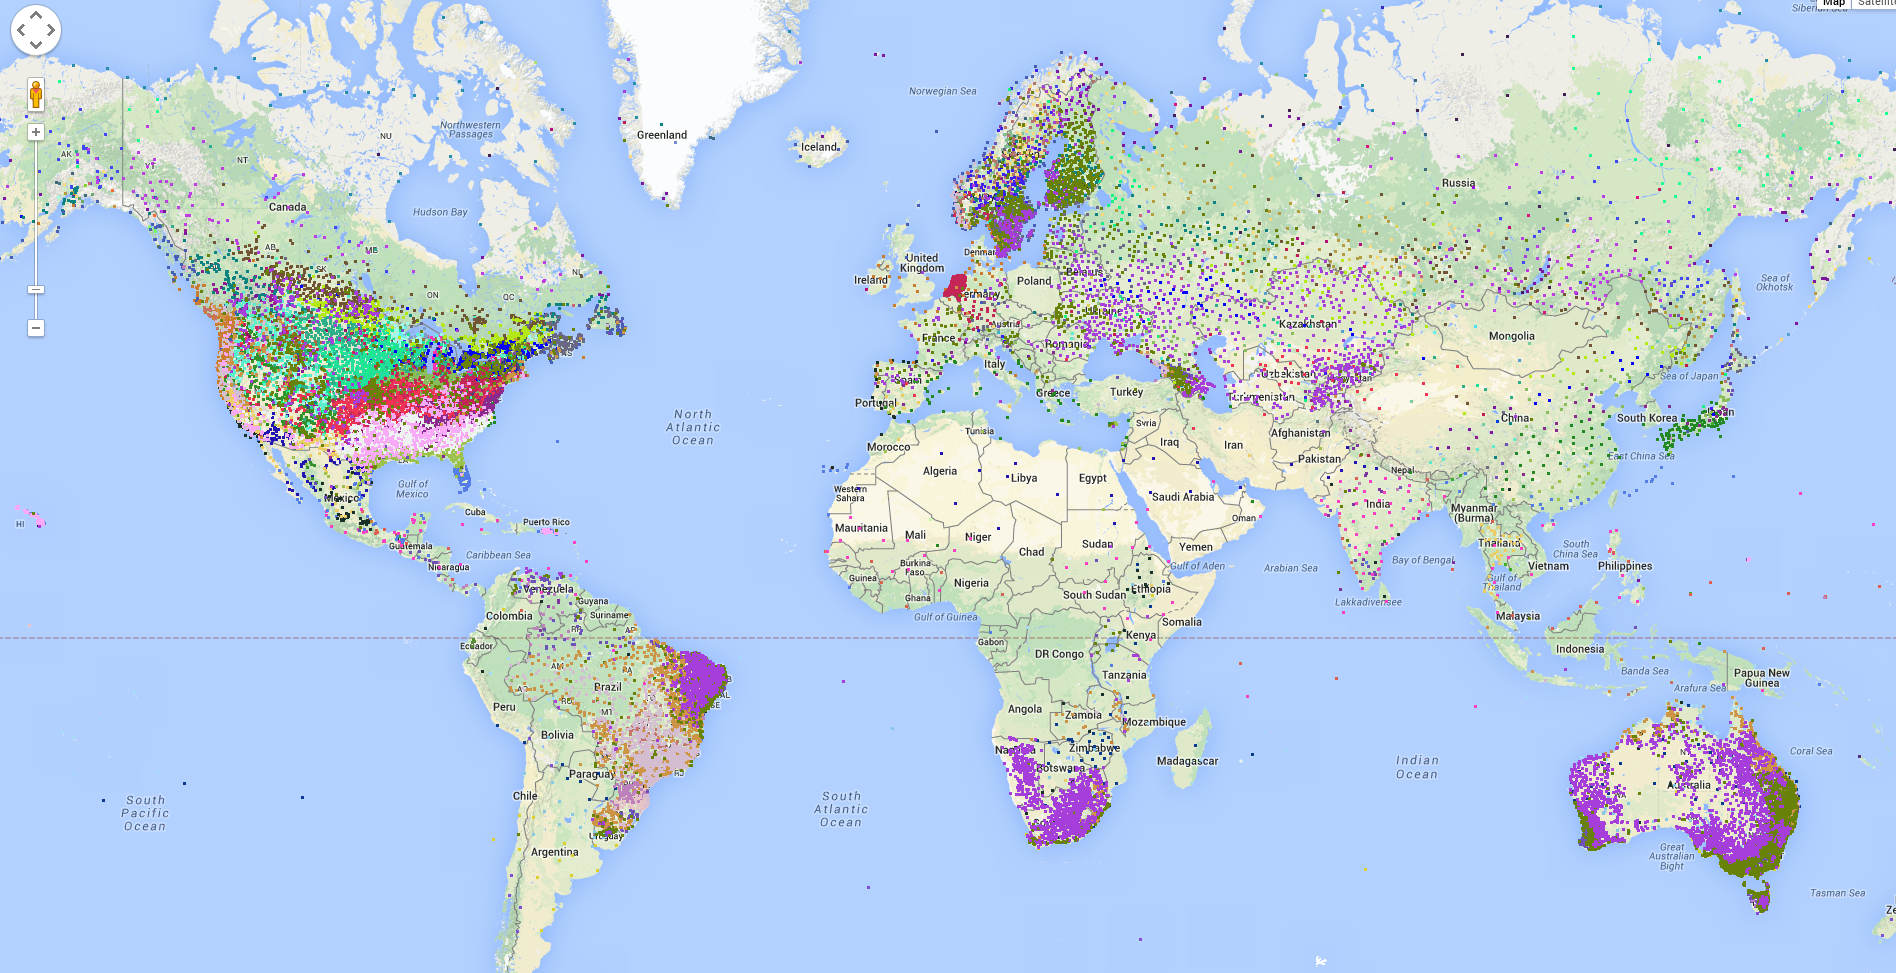
\includegraphics[width =.65\linewidth]{images/1983.png}\\1983\\
        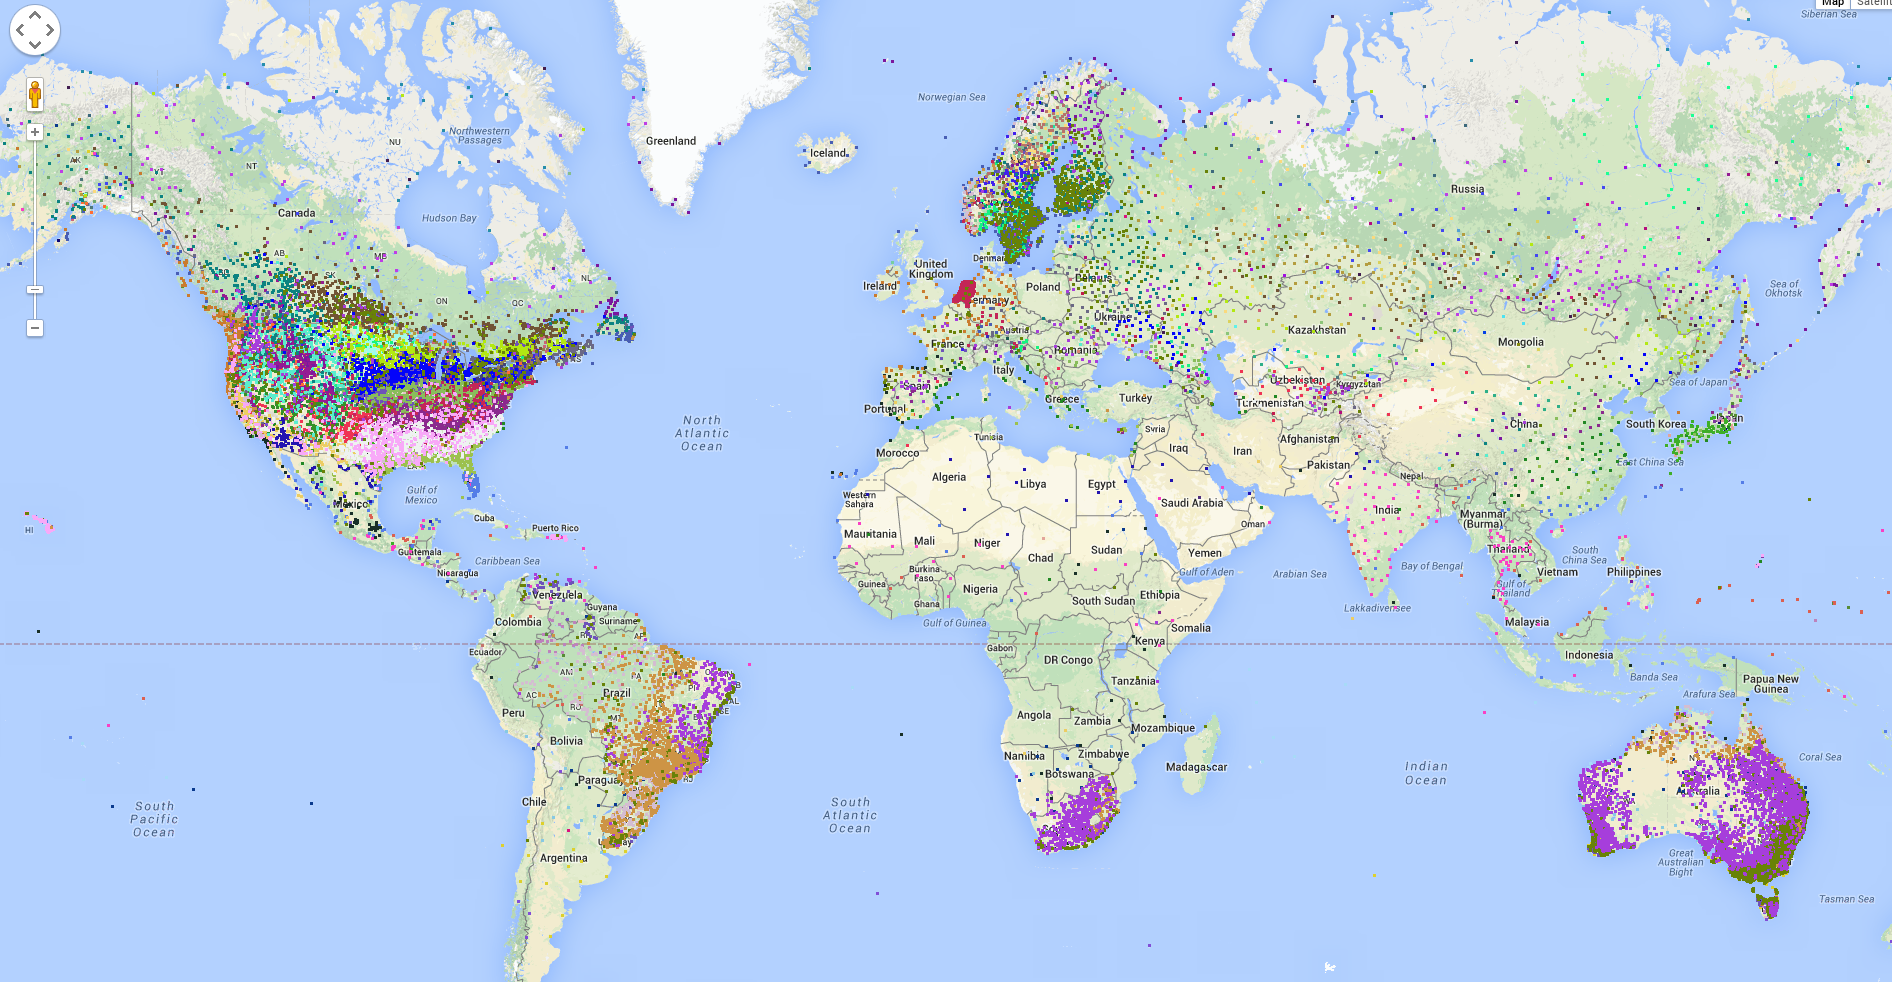
\includegraphics[width =.65\linewidth]{images/1993.png}\\1993\\
        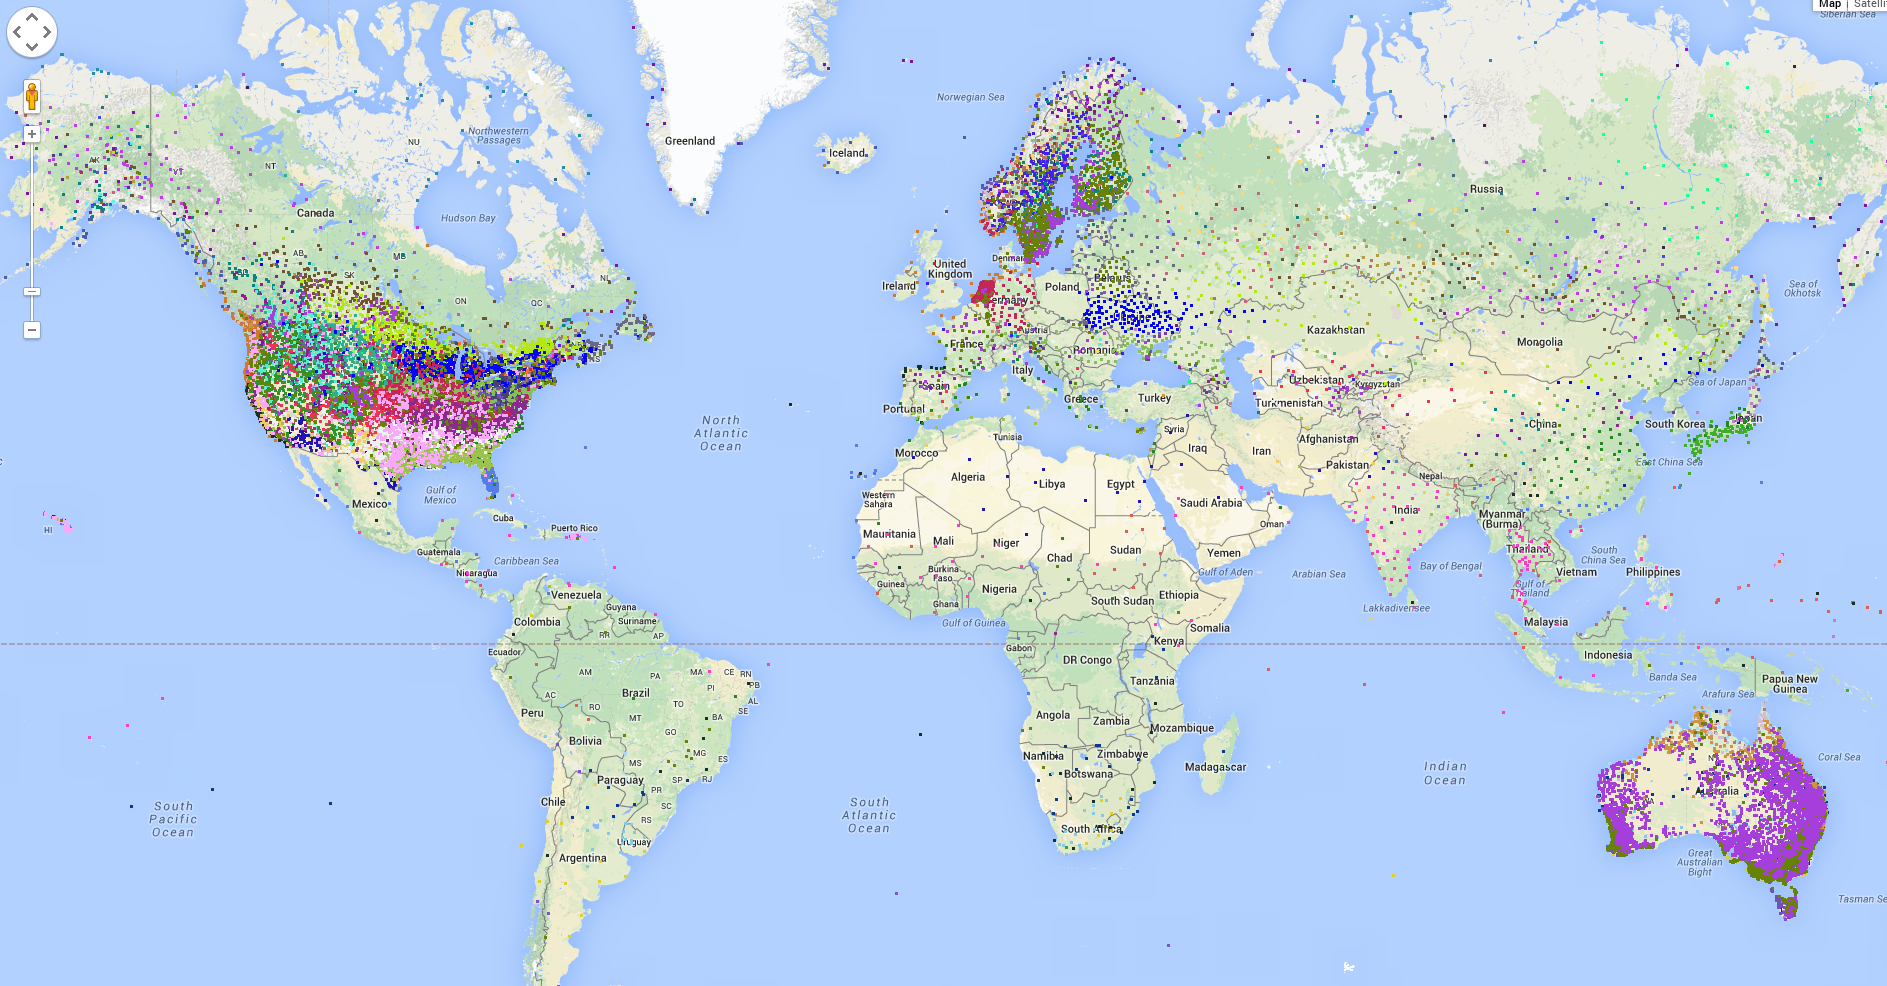
\includegraphics[width =.65\linewidth]{images/2003.png}\\2003\\
        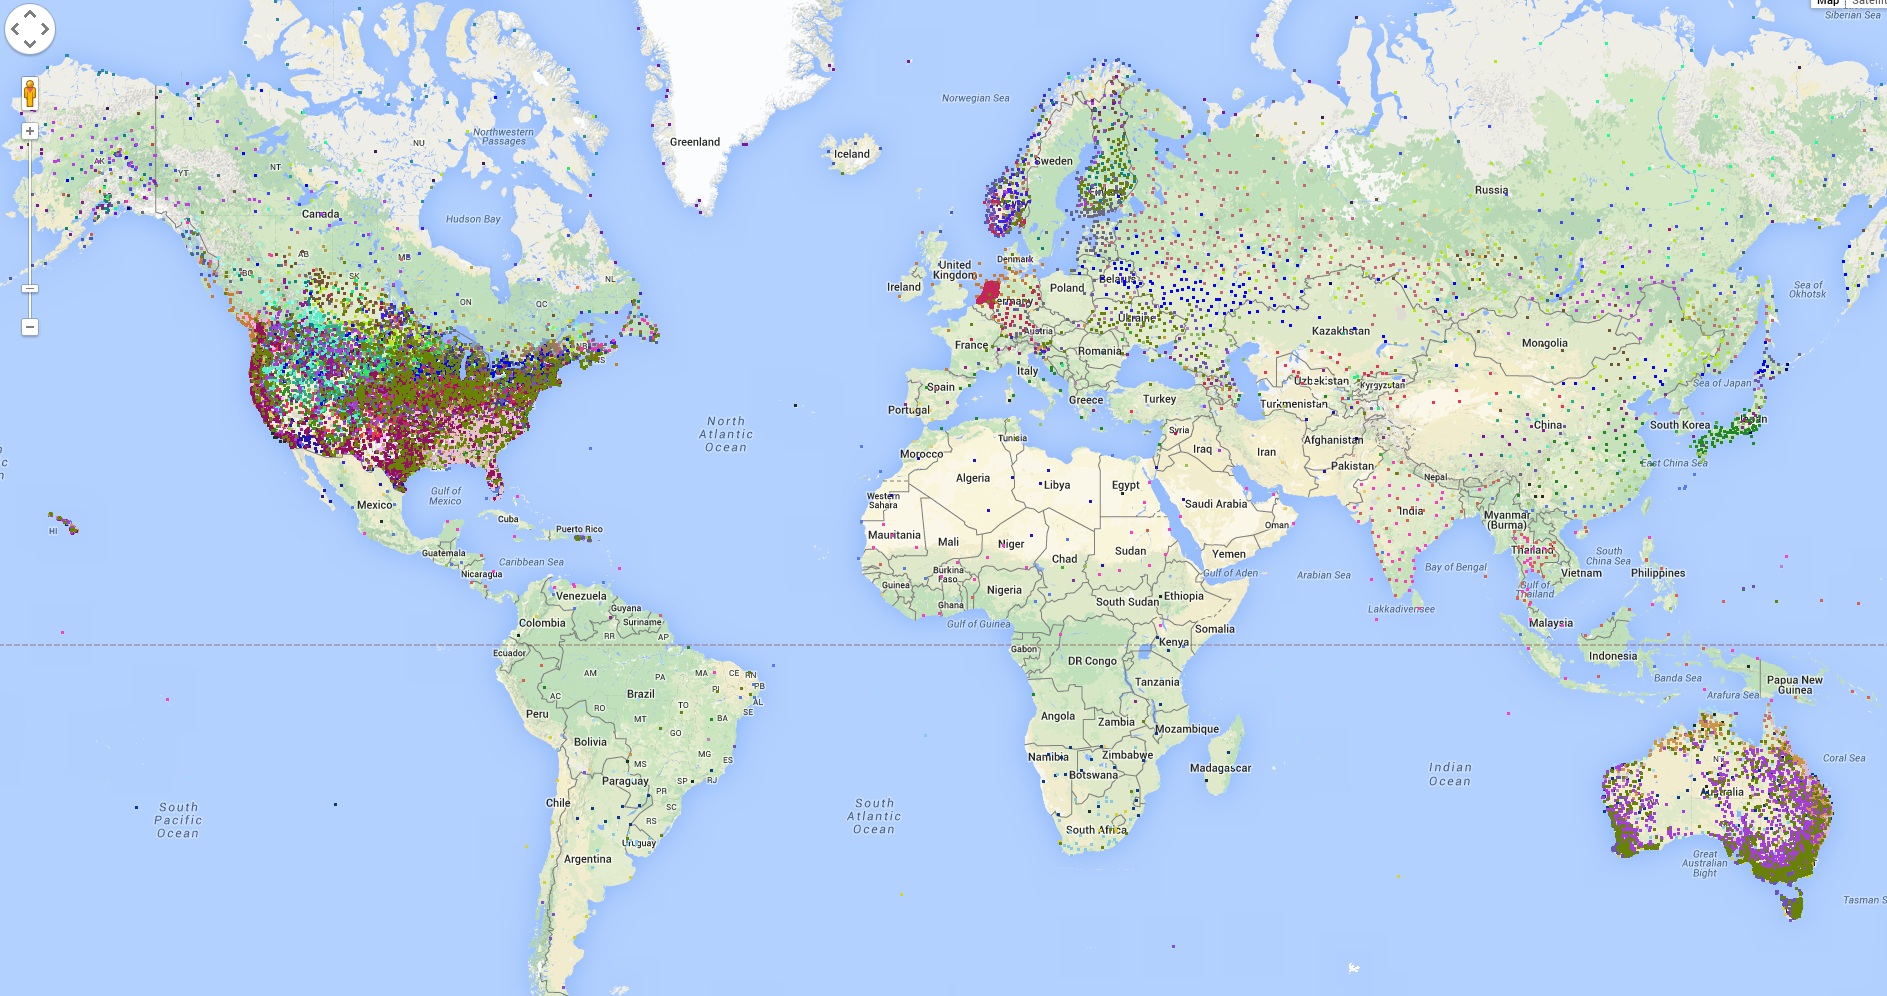
\includegraphics[width =.65\linewidth]{images/2013.png}\\2013\\
    \end{tabular}
    \caption{Clustering results of four different years.}
\end{figure}

\subsection{Result of more than a century}

Also, adjusted the parameter again 90 clusters, 500 iterations to see if there is any similar pattern.

The results before $1876$ is meaningless since there were not enough data.
\begin{figure}
    \centering
    \begin{tabular}{c}
        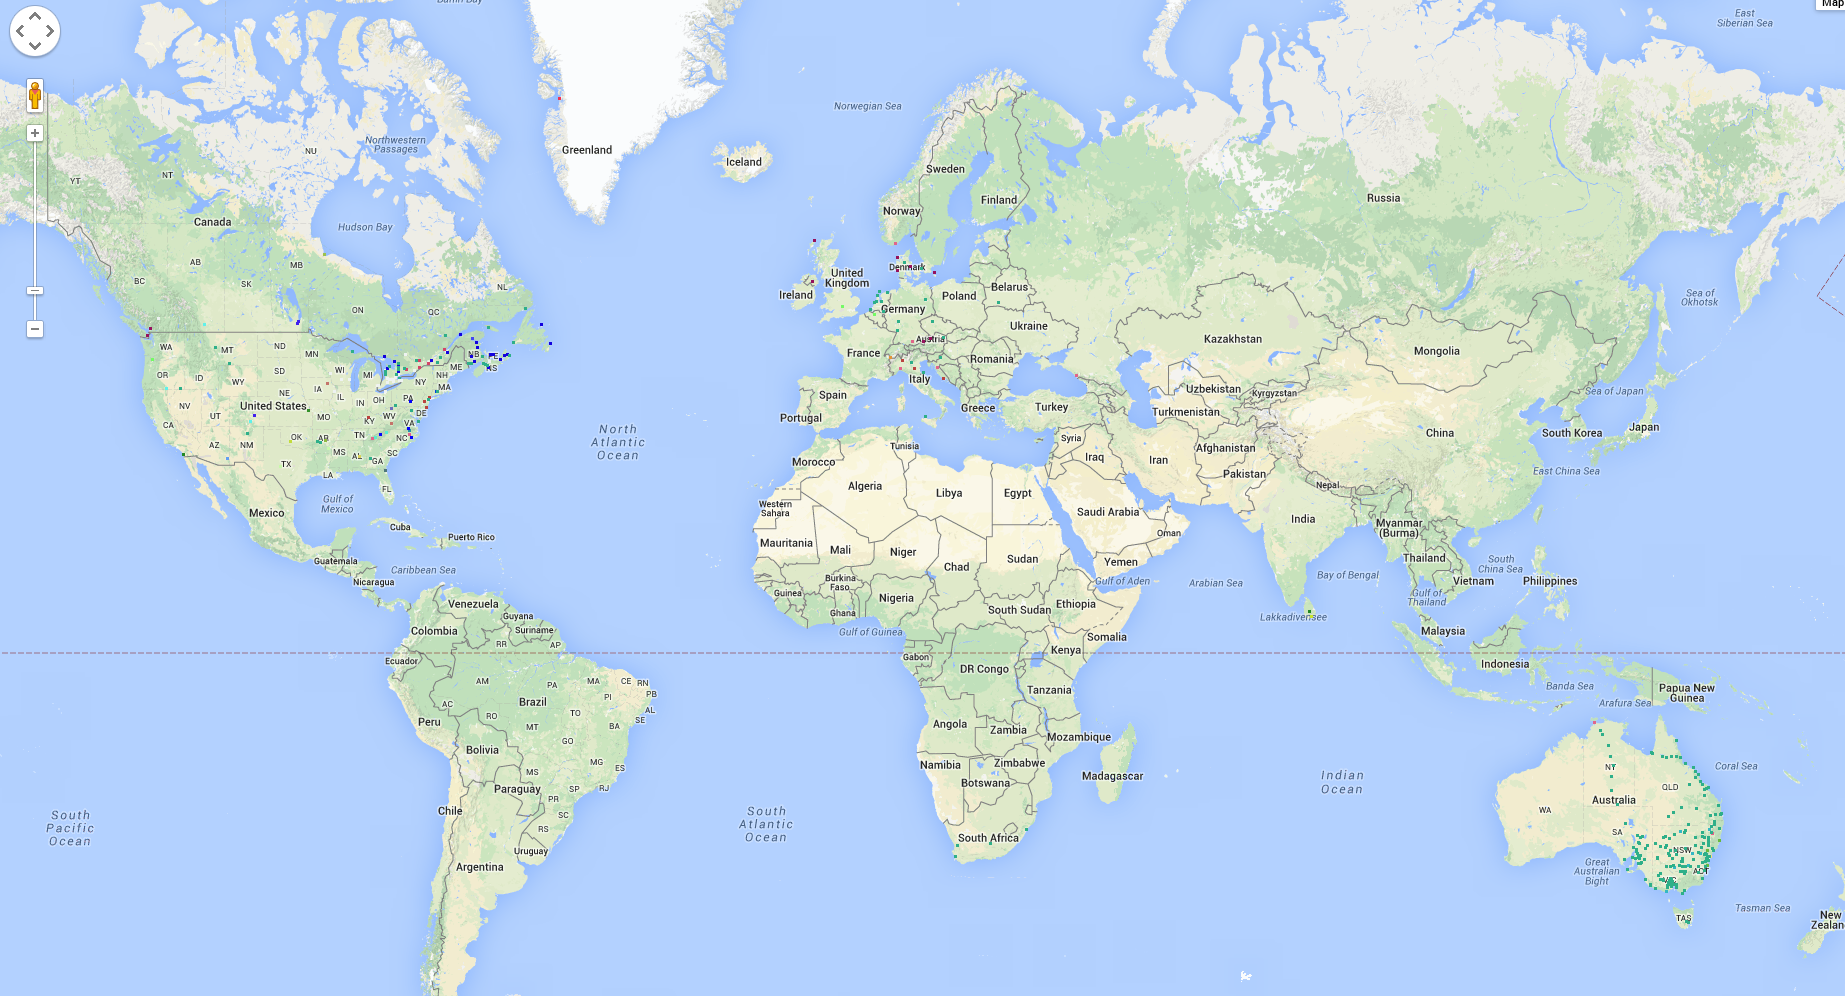
\includegraphics[width =.65\linewidth]{images/1876.png}\\ 1876\\
        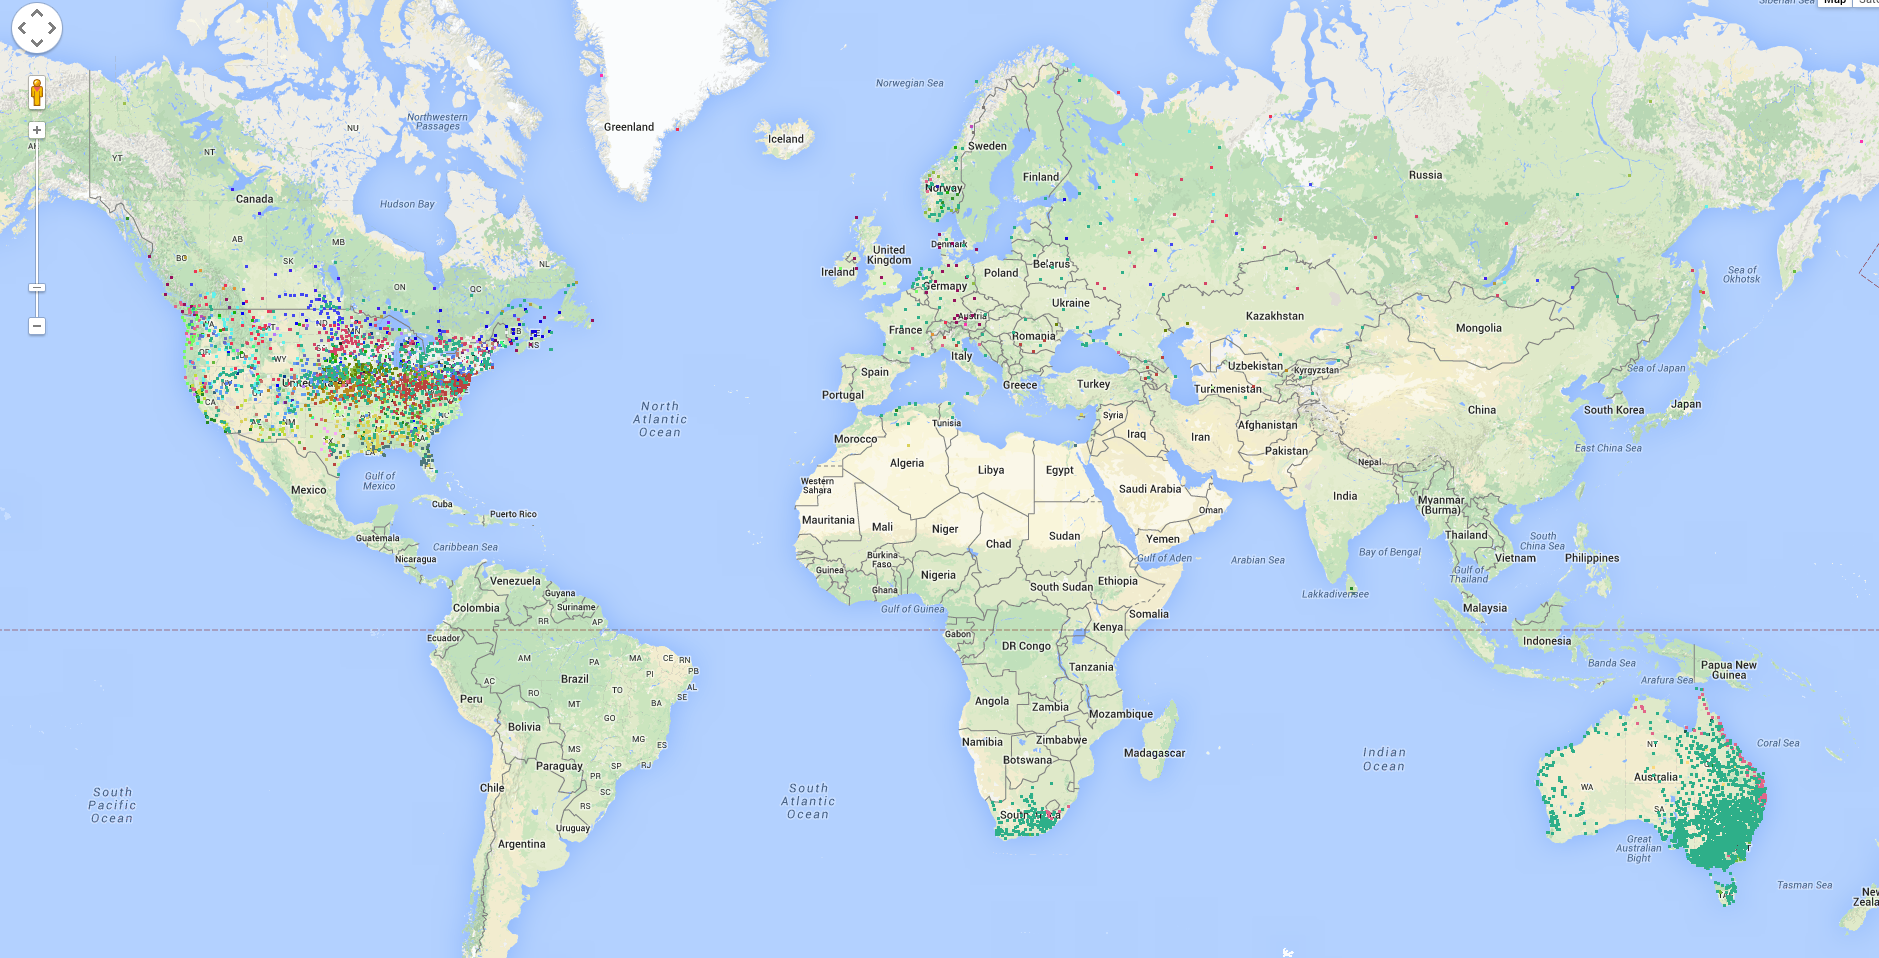
\includegraphics[width =.65\linewidth]{images/1896.png}\\ 1896\\
        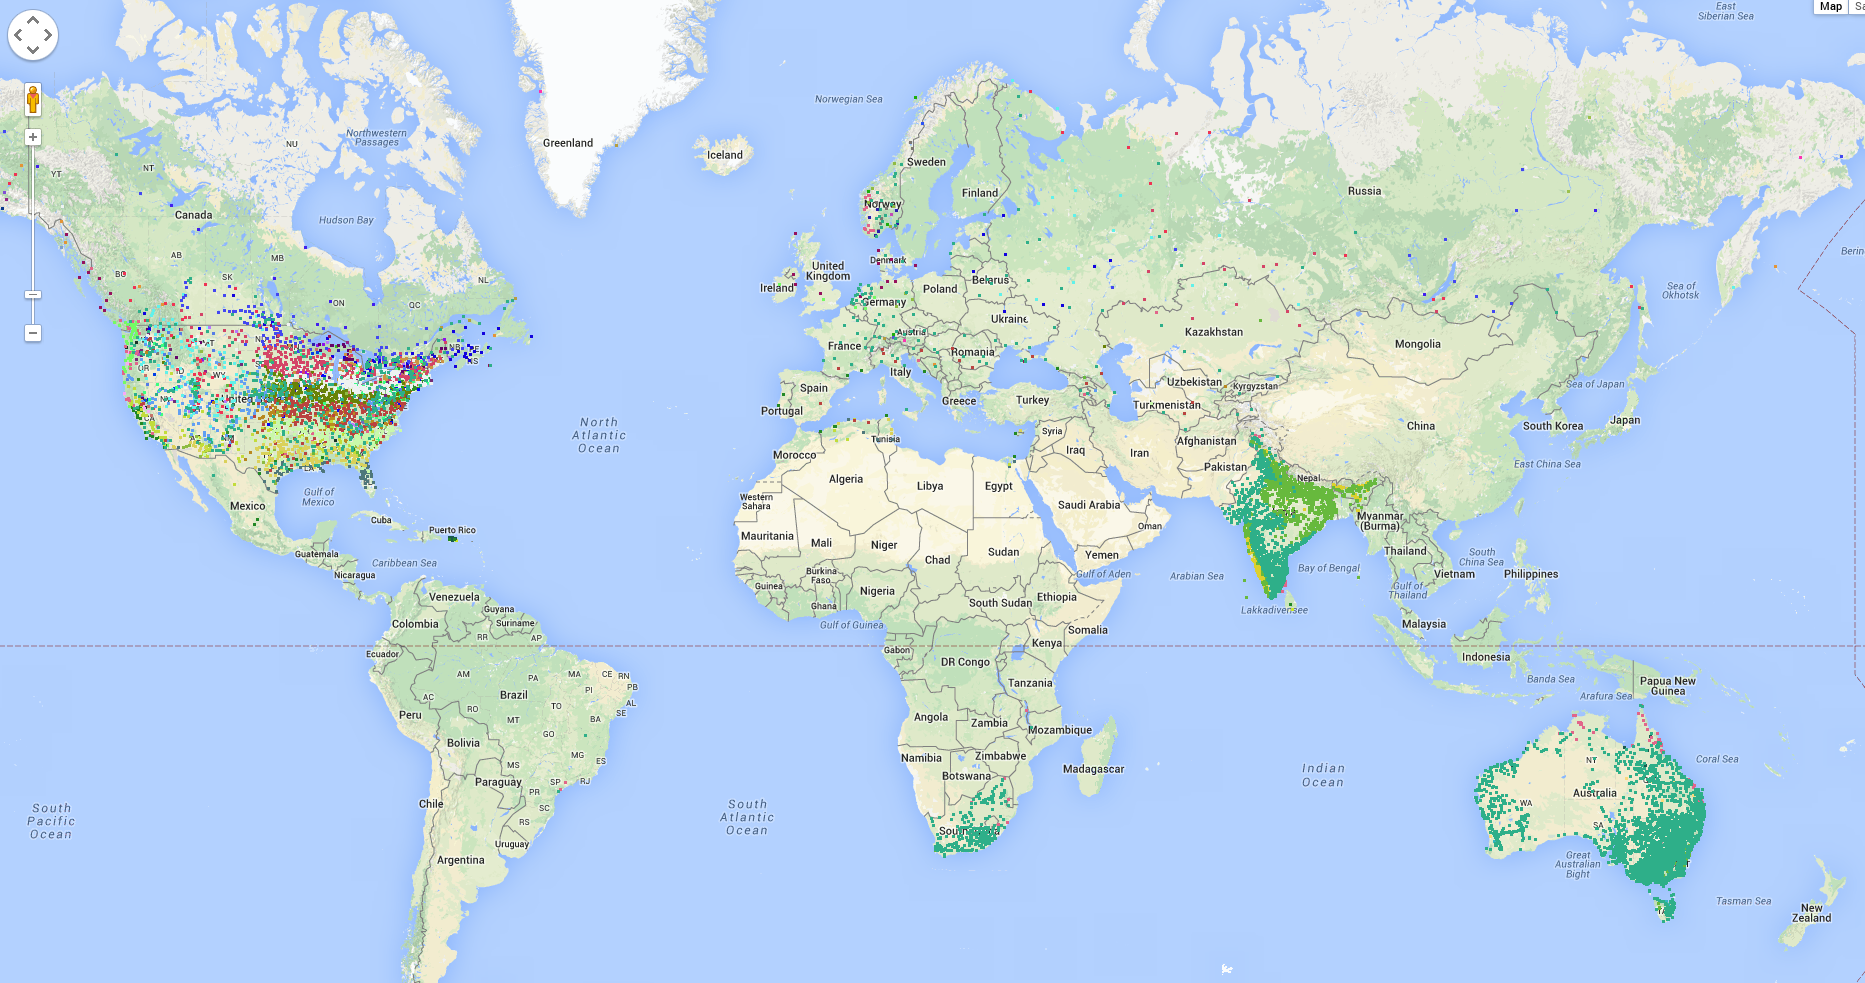
\includegraphics[width =.65\linewidth]{images/1904.png}\\ 1904\\
        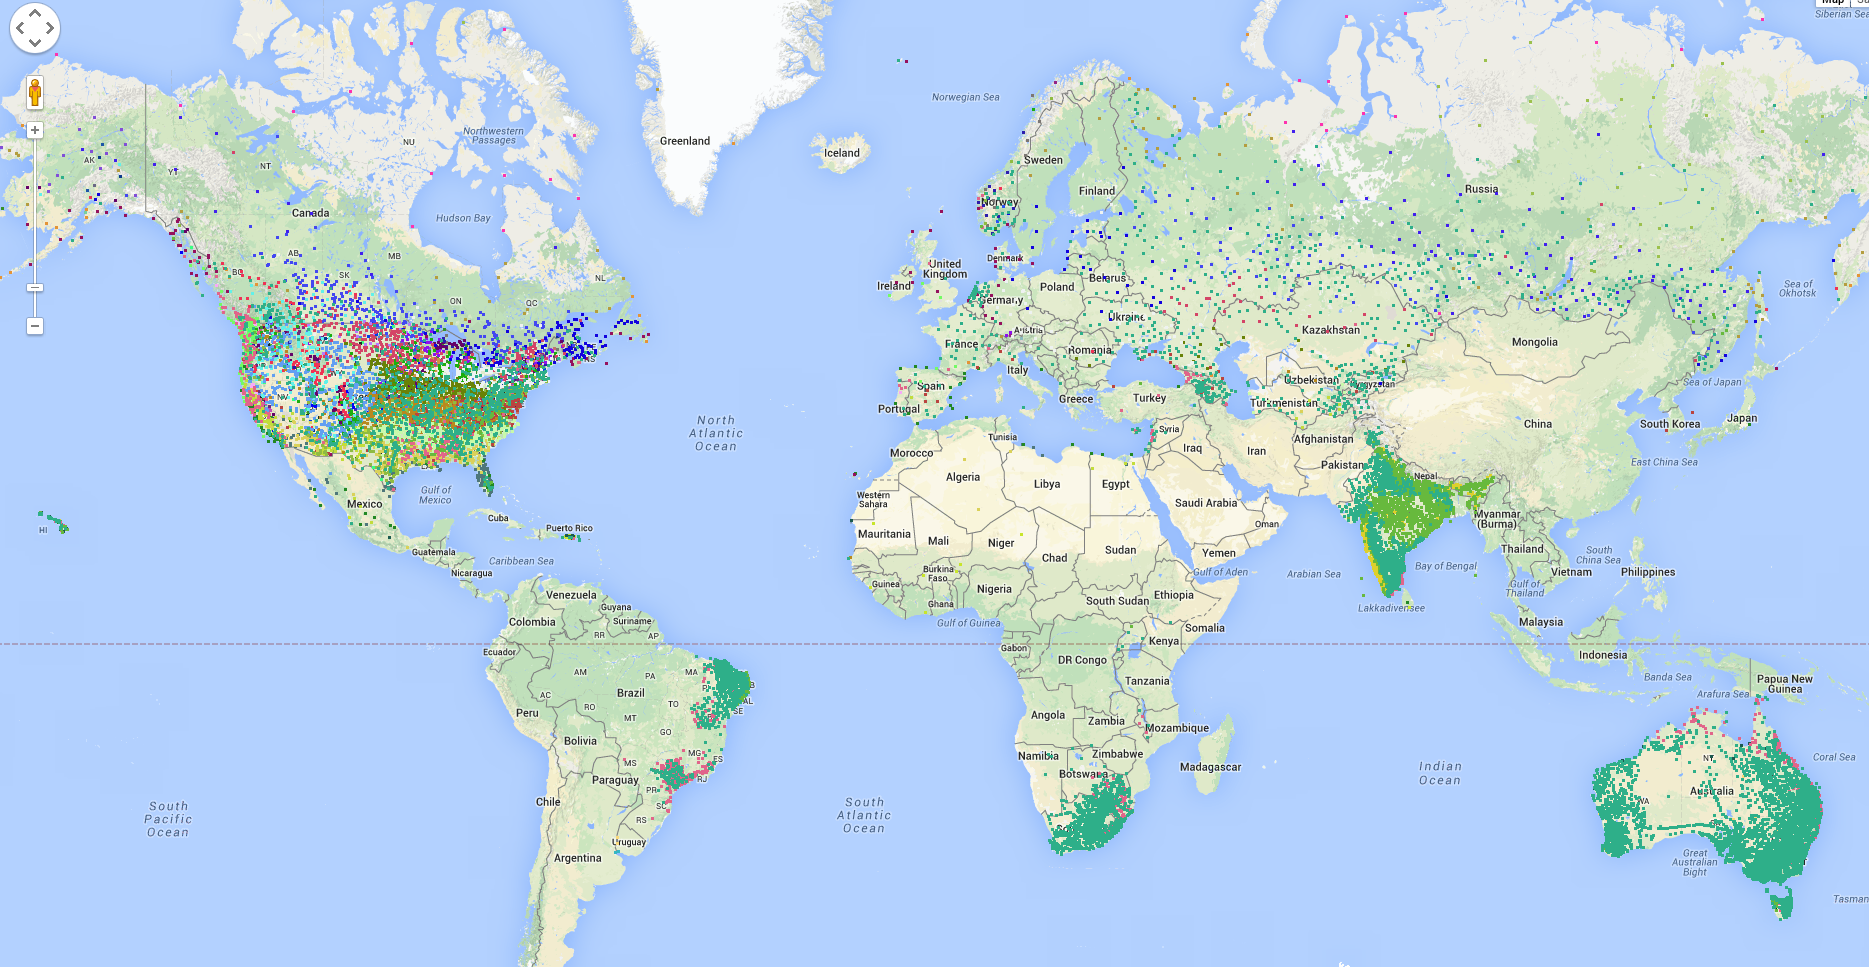
\includegraphics[width =.65\linewidth]{images/1940.png}\\ 1940\\
        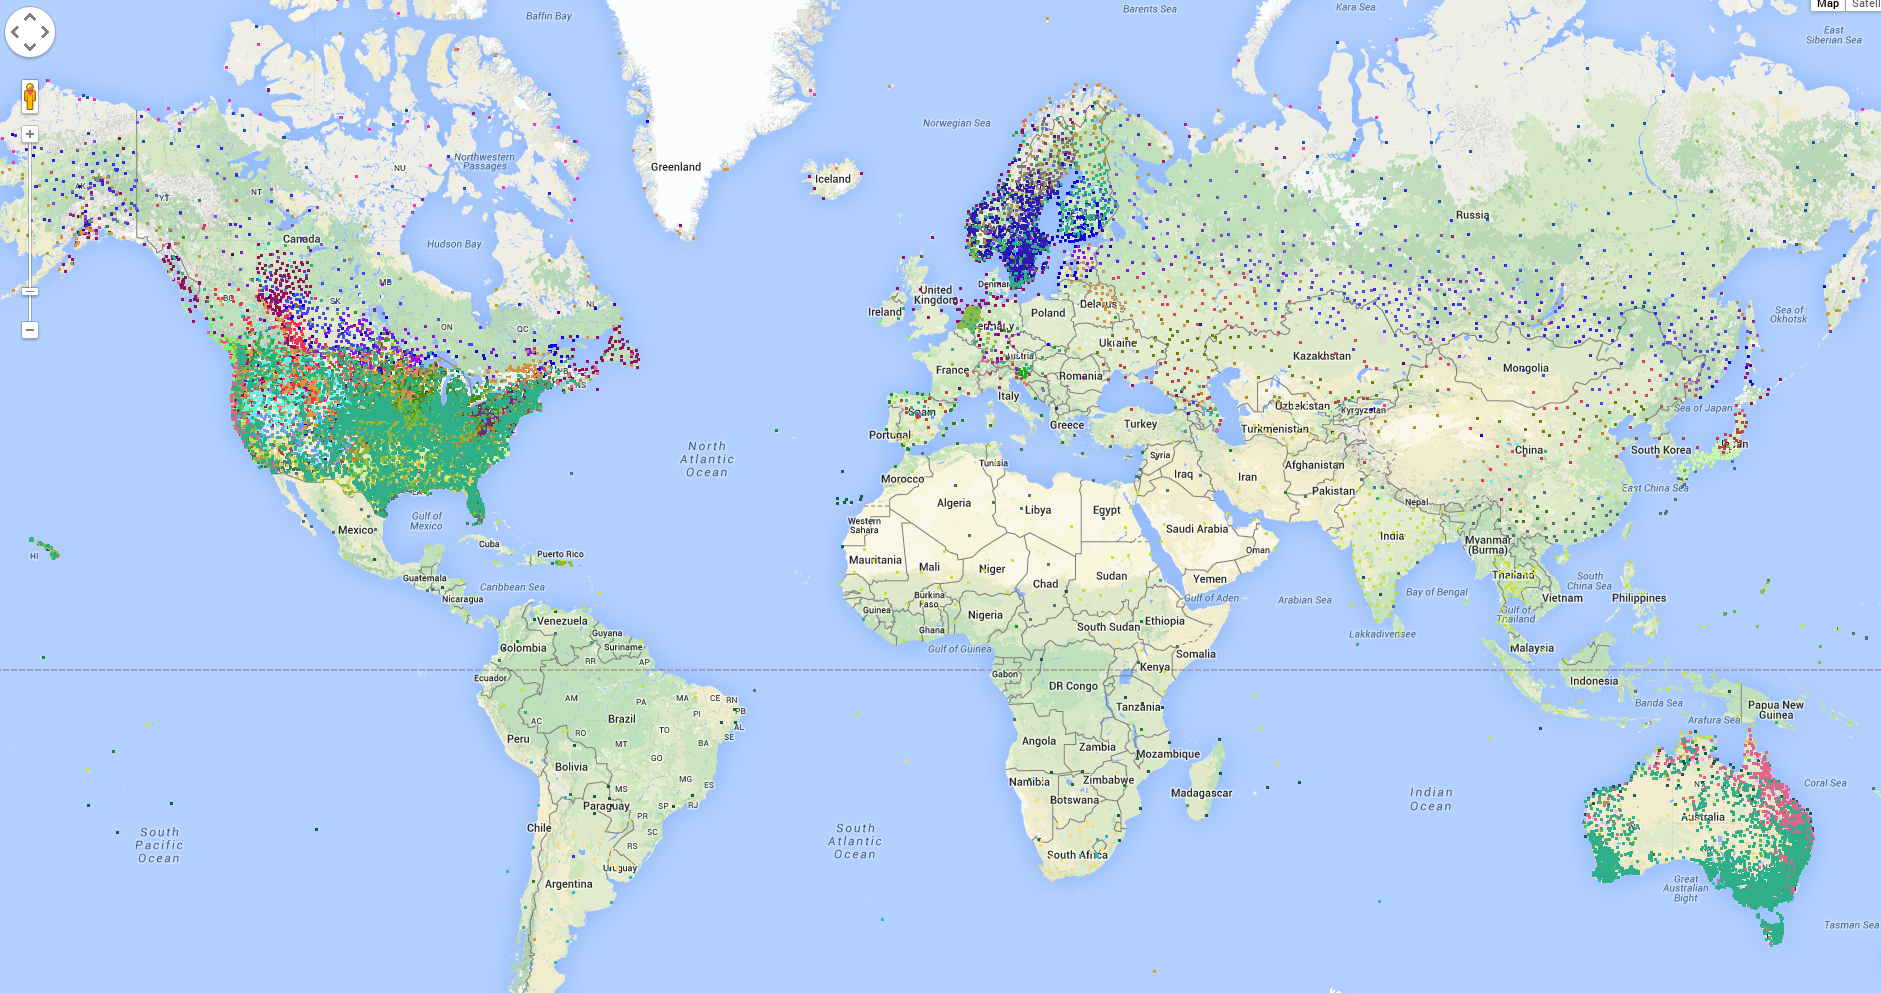
\includegraphics[width =.65\linewidth]{images/2010.png}\\ 2010\\
    \end{tabular}
    \caption{Clustering results over a century.}
\end{figure}

